\documentclass[9pt,twocolumn,twoside,pdftex]{optica}


\newtheorem{definition}{Definition}

\setboolean{shortarticle}{false}
\setboolean{minireview}{false}



\title{Dual oxygen and temperature luminescence sensor based on artificial intelligence}

\author[1,2,*]{Francesca Venturini}
\author[2]{Umberto Michelucci}
\author[1]{Michael Baumgartner}

\affil[1]{Institute of Applied Mathematics and Physics, Zurich University of Applied Sciences,
Technikumstrasse 9, 8401 Winterthur, Switzerland}
\affil[2]{TOELT LLC; Birchlenstr. 25, 8600 Dübendorf, Switzerland}

\affil[*]{Corresponding author: francesca.venturini@zhaw.ch}




% To be edited by editor
% \dates{Compiled \today}

%\ociscodes{(140.3490) Lasers, distributed feedback; (060.2420) Fibers, polarization-maintaining; (060.3735) Fiber Bragg gratings.}
%300.6280   Spectroscopy, fluorescence and luminescence
%260.3800   Luminescence
%120.0280   Remote sensing and sensors
%100.4996   Pattern recognition, neural networks
%200.4260   Neural networks
%https://www.osapublishing.org/submit/ocis/#230.0230
% To be edited by editor
% \doi{\url{http://dx.doi.org/10.1364/optica.XX.XXXXXX}}

\begin{abstract}

A well-known optical approach to measure oxygen partial pressure is the quenching of luminescence by the oxygen molecules. Sensors based on this principle typically rely on approximate empirical models to parametrise the dependence of the sensing quantity on influencing factors, like the temperature. In this work, we propose a new artificial intelligence neural network approach which allows the extraction of both the oxygen concentration and the temperature using one single dye molecule and measuring a single quantity, namely the decay time. The results demonstrate that firstly, using neural networks it is possible to extract both the oxygen concentration and the temperature from the measurement of one single quantity and using one single indicator; secondly, that the use the proposed neural networks networks allow more accurate and stable predictions for both the parameters. Furthermore, the proposed artificial intelligence approach is not limited to oxygen and temperature sensing, but can be applied to luminescence of multiple indicators, whenever the underlying mathematical model is not known or too complex to derive the desired quantities from a single measurement.

\end{abstract}

\setboolean{displaycopyright}{true}

\begin{document}

\maketitle

\section{Introduction}

The simultaneous determination of multiple parameters can be very advantageous in many sensor applications, for example when in-situ or remote acquisition is required. If the measured parameters are interdependent, their simultaneous determination becomes a necessity. Optical  luminescence sensing has the advantage of enabling multiple sensing, since the same optical elements, like optical fiber and detector, can be used therefore allowing a compact and easy sensor design. The typical approaches are based on either the use of a single luminescence indicator (luminophore), whose luminescence is sensitive to more than one parameters, or the use of several luminophores, one for each parameter, all embedded in a substrate in a close physical proximity \cite{Stich2010,Wang2014}. To be able to determine each parameter separately it is usually necessary to determine more than one optical property (e.g., absorption spectrum, emission spectrum, luminescence intensity, decay time) or to use special detection schemes to take advantage of the differences of one optical property of the used luminophores \cite{Collier2013,Wang2014}. 

PROBLEMA PARTICOL RILEVANTE PER OSSIGENO

The determination of oxygen partial pressure is of great interest in numerous areas, like medicine, biotechnology, and chemistry. 
The most used optical measuring approach uses the effect of the quenching of luminescence by the oxygen molecules. The measuring principle is based on the measurement of the luminescence of a specific molecule or luminophore, whose intensity and decay time are reduced due to collisions with molecular oxygen \cite{Lakowicz2006}.

Sensors based on this principle typically rely on approximate empirical models to parametrise the dependence of the sensing quantity on influencing factors. A new approach is to use feed-forward neural networks to predict the desired variables. Unfortunately, those kind of networks usually perform less efficiently when applied to multi-dimensional regression problems. In this work, we propose a new multi-task learning (MTL) neural network approach which allows the extraction of both the oxygen concentration and the temperature using one single indicator and measuring a single quantity, namely the decay time. The results demonstrate that firstly, using neural networks it is in principle possible to extract both the oxygen concentration and the temperature from the measurement of one single quantity and using one single indicator; secondly, that the use the proposed MTL networks allow more accurate and stable predictions for both the parameters. Furthermore, the proposed MTL approach is not limited to luminescence quenching but may be of particular relevance in all those cases, where the mathematical model is not known, too complex or not really of interest and the only goal of the regression problem is to build a system that is able to determine as accurately as possible.


IDEE
Temperature is a key parameter in numerous fields of science and technology. While not a chemical parameter by itself, its knowledge is of highest significance since temperature affects the response of all chemical sensors
Knowing temperature is particularly important in fluorescent sensing of oxygen since quenching by oxygen always is highly temperature dependent
Pressure Sensitive Paint: any method requires correction due to the temperature dependence of the luminescence of the paint, for example non-oxygen quenched,  temperature-dependent  phosphor  is  added  to  the  standard  paint

\section{Methods}
\label{sec:methods}

\subsection{Luminescence Quenching for Oxygen Determination}
\label{Theory}

Luminescence-based oxygen sensors usually consist of a dye molecule (luminophore) whose luminescence intensity and decay time decrease depending on the O$_2$ concentration. This reduction is due to collisions of the excited luminophore with molecular oxygen, which thus provide a radiationless deactivation process (collisional quenching). 
In the case of homogeneous media characterized by an intensity decay which is a single exponential, the decrease in intensity and lifetime are both described by the Stern-Volmer (SV) equation \cite{Lakowicz2006}
\begin{equation}
\frac{I_0}{I}=\frac{\tau_0}{\tau}=1+K_{SV} \cdot \left[O_2\right]
\label{SVe}
\end{equation}
where $I_0$ and $I$, respectively, are the luminescence intensities in the absence and presence of oxygen, $\tau_0$ and $\tau$ the decay times in the absence and presence of oxygen, $K_{SV}$ the Stern–Volmer constant and $\left[O_2\right]$ indicates the oxygen concentration.

For practical applications, the luminophore needs to be embedded in a supporting substrate, frequently a polymer. As a result, the SV curve deviates from the linear behavior of equation (\ref{SVe}). This deviation can be due, for example, to heterogeneities of the micro-environment of the luminescent indicator, or the presence of static quenching \cite{Wang2014}. A scenario which describes this non-linear behavior involves the presence in the substrate of at two or more environments, in which the indicator is quenched at different rates \cite{Carraway1991,Demas1995}. This multi-site model describes the SV curve as the sum of two or more
\begin{equation}
%\frac{I_0}{I}=\bigg( \frac{f}{1+K_{SV1} \cdot \left[O_2\right]}+\frac{1-f}{1+K_{SV2}\cdot \left[O_2\right]}\bigg)^{-1}
\frac{I_0}{I}=\bigg[
\frac{f_i}{1+K_{SV,i} \cdot \left[O_2\right]}
\bigg]^{-1}
\label{SVe2}
\end{equation}
where $I_0$ and $I$, respectively, are the luminescence intensities in the absence and presence of oxygen, $f_i$'s are the fractions of the total emission for each component under unquenched conditions, $K_{SVi}$'s are the associated effective Stern–Volmer constants, and $\left[O_2\right]$ indicates the oxygen concentration. A simplification of this model is that one of the sites is not quenched and therefore the constant $K_{SV2}$ is zero.
 Depending on the luminophore and on the substrate material, the proposed model may be even more complex \cite{Demas1995,Hartmann1995,Mills1999}.

Since in most industrial and commercial sensor applications, the decay time $\tau$ is frequently preferred to intensity measurement because of its higher reliability and robustness. The determination of the decay time is done most easily in the frequency domain by modulating the intensity of the excitation.  As a result, the emitted luminescence is also modulated but shows a phase shift $\theta$ due to the finite lifetime of the excited state. This method, has the advantage of allowing very simple and low-cost realization and is widely used in commercial applications.

Although the multi-site model was introduced for luminescence intensities, it is frequently also used to describe the oxygen dependence of the decay times \cite{Demas1995,Quaranta2012}. Therefore, in the simplest case of a two-sites scenario, the model can be rewritten in terms of phase shift as \cite{Michelucci2019}
\begin{equation}
\begin{aligned}
\frac{\tan \theta (\omega, T, [O_2])}{\tan \theta_0 (\omega, T)} =& \bigg( \frac{f (\omega , T) }{1+K_{SV1} (\omega , T) \cdot \left[O_2\right]}+ \\
&\frac{1-f (\omega , T) }{1+K_{SV2} (\omega , T) \cdot \left[O_2\right]} \bigg)^{-1} \\
\label{theta_full}
\end{aligned}
\end{equation}
where $\theta_0$ and $\theta$, respectively, are the phase shifts in the absence and presence of oxygen, $f$ and $1-f$ are the fractions of the total emission for each component under unquenched conditions, $K_{SV1}$ and $K_{SV2}$ are the associated Stern–Volmer constants for each component, and $\left[O_2\right]$ indicates the oxygen concentration. It is to be noted that the quantities $\theta_0$, $f$, $K_{SV1}$, and $K_{SV2}$ are all non-linearly temperature dependent and may result frequency dependent, an artifact of the approximation of the model. Finally, Eq. \ref{theta_full} needs to be inverted to determine $[O_2]$ from the measured quantity $\theta$.


\subsection{Experimental Setup}
\label{Experimental}


The optical setup used in this work for the luminescence measurements is shown schematically in Fig. \ref{fig:setup}. To be able to acquire a large number of data, both the software for the instrument control and for the data acquisition was written using LabVIEW by National Instruments. The acquisition procedure is described in detail in Sect.\ref{Data}.

\begin{figure}[htbp]
\centering
\includegraphics[keepaspectratio, width=8.5cm]{setup_auto.eps}
\caption{Scheme of the optical experimental setup. Blue is the excitation, red the luminescence optical path. SP: short pass filter; LP: long pass filter PD: photodiode; TIA: trans-impedance amplifier.}
\label{fig:setup}
\end{figure}

The sample used for the characterization and test is a commercially available Pt-TFPP-based oxygen sensor spot (PSt3, PreSens Precision Sensing GmbH).
To control the temperature of the samples, these were placed in good thermal contact with a copper plate, placed in a thermally insulated chamber. The temperature of this plate was adjusted using a Peltier element and stabilized with a temperature controller (PTC10, Stanford Research Systems). The thermally insulated chamber was connected to a self-made gas-mixing apparatus which enabled to vary the oxygen concentration between 0 $\%$ and 20 $\%$ vol $O_2$ by mixing nitrogen and dry air from two bottles. In the following, the concentration of oxygen will be given in $\%$ of the oxygen concentration of dry air and indicated with $\%$ air. This means, for example, that 20 $\%$ air corresponds to 4 $\%$ vol $O_2$ and 100 $\%$ air corresponds to 20 $\%$ vol $O_2$. The absolute error on the oxygen concentration adjusted with the gas mixing device is estimated to be below 1 $\%$ air. 
 
The excitation light was provided by a 405 nm LED (VAOL-5EUV0T4, VCC Visual Communications Company LLC), filtered by a an short pass (SP) filter with cut-off at 498 nm (Semrock 498 SP Bright Line HC short pass) and focused on the surface of the samples with a collimation lens (EO43987, Edmund Optics). The luminescence was focussed by a lens (G063020000, LINOS) and collected by a photodiode (SFH 213 Osram).
To suppress stray light and light reflected by the sample surface, the emission channel was equipped with a long pass filter with cut-off at 594 nm (Semrock 594 LP Edge Basic long pass) and a short pass filter with cut-off at 682 nm (Semrock 682 SP Bright Line HC short pass). The driver for the LED and the trans-impedance amplifier (TIA) are self-made.
For the frequency generation and the phase detection a two-phase lock-in amplifier (SR830, Stanford Research Inc.) was used. 

\subsection{Automated Data Acquisition}
\label{Data}

The series of measurements were carried out following the flow shown in Fig. \ref{fig:auto-data}. First the acquisition program fixed the temperature and concentration. Then the phase-shift was measured for varying the modulation frequency between 200 Hz and 15000 kHz. This measurement was repeated 20 times. Next, keeping the temperature fixed, the program changed the oxygen concentration and the entire frequency-loop was repeated.
The oxygen concentration was varied between 0 $\%$ air and 100 $\%$ air in 5 $\%$ steps.
Finally, the temperature is changed and then the oxygen and frequency loops where repeated. The temperature was varied between 5 $^\circ$C and 45 $^\circ$C in 5 $^\circ$C steps.
The total number of measurements is thus 50 x 20 x 21 x 9 = 189000 which required approximately 65 hours. This number of measurement was chosen as a compromise between maximizing the number of data for the training of the neural network and avoiding photodegradation, which naturally occurs when the sample is subjected to illumination. A the end of the session a minimal change in the phase shift was observed (QUANTIFY?)

\begin{figure}[t!]
\centering
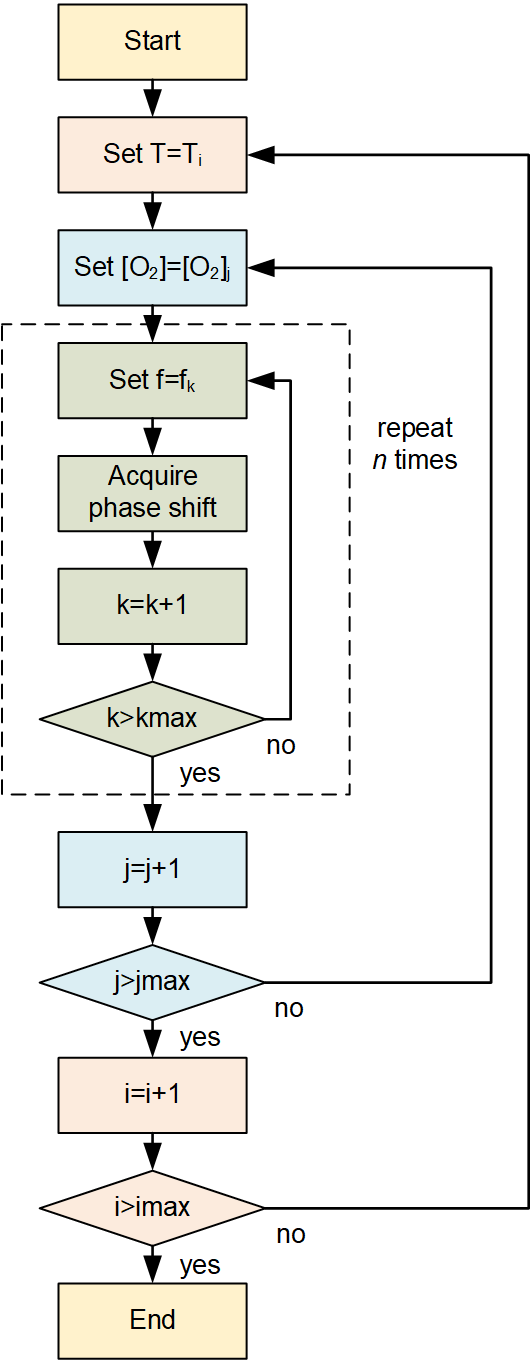
\includegraphics[keepaspectratio, width=6 cm]{flow-chart.png}
\caption{Flow-chart of the automatic measurement process.}
\label{fig:auto-data}
\end{figure}

%%%%%%% UMBI

\subsection{Neural Network Software}
\label{NN}



The software component of this new sensor type is based on a neural network model (NNM). A NNM is made of three components \cite{Michelucci2017}: a neural network architecture (that includes how neurons are connected, the activation functions and all the hyperparameters), a loss function (that we will indicate with $L$) and an optimiser algorithm. In this section those three components are described in detail.

\subsubsection{Neural Network Architecture}

The artificial network used in this work has a multi-task-learning architecture and is depicted in Figure \ref{fig:NN_MTL_O2_T}. It consists of three common hidden layers with 50 neurons each which generate as output a "shared representation". The name comes from the fact that the output of those layers is used to evaluate both $[O_2]$ and $T$. These are followed by three branches, two with each two additional "task-specific hidden layers" to predict respectively $[O_2]$ and $T$, and then one without additional layers to predict $[O_2]$ and $T$ at the same time.The shared representation is the input of two "task-specific hidden layers", that learn how to predict $[O_2]$ and $T$ better. This architecture uses the common hidden layers to find common features beneficial to each of the two tasks. During the training phase, learning to predict $[O_2]$ will influence the common hidden layers and therefore, the prediction of $T$, and vice-versa. The further task-specific hidden layers learn specific features to each output and therefore improve the prediction accuracy. The number of neurons of each task-specific hidden layer is 5.

As activation function the sigmoid activation functions was used for all the neurons. For all the runs presented in this article a learning rate of $\gamma = 10^{-3}$ has been used. Number of epochs and mini-batch size has been varied to optimize the NNM performance and are discussed in the appropriate sections.

\subsubsection{Loss Function}

The loss function used in this work is the mean square error (MSE), which is defined as
\begin{equation}
MSE = \frac{1}{n}\sum_{j=1}^n \sum_{k=1}^d (y_k^{[j]}-\hat y_k^{[j]})^2
\label{MSE}
\end{equation}
where $n$ is the number of observations in the input dataset; ${\mathbold y}^{[j]} \in \mathbb{R}^d$ is the measured value of the desired quantity for the $j^{th}$ observation (indicated as a superscript between square brackets), with $j=1, ..., n$; $ \hat {\mathbold y}^{[j]} \in \mathbb{R}^d$ is the output of the network, when evaluated on the $j^{th}$ observation.T Since there are multiple branches, a global cost function $L$ needs to be defined as a linear combination of the task-specific cost functions with weights $\alpha_i$ will be minimized
\begin{equation}
L = \sum_{i=1}^{n_T}\alpha_i L_i .
\label{globalcf}
\end{equation}
The parameters $\alpha_i$ have to be determined during the hyper-parameter tuning phase to optimize the network predictions.
In this paper, being the cost function the MSE (Equation \ref{MSE}), the global cost function of Equation \ref{globalcf} is
\begin{equation}
L = \sum_{i=1}^{n_T}\alpha_i \frac{1}{n}\sum_{j=1}^n \sum_{k=1}^d (y_k^{[j]}-\hat y_k^{[j]})^2
\end{equation}
where  $n_T$ is the number of tasks; $n$ is the number of observations in the input dataset; ${\mathbold y}^{[j]} \in \mathbb{R}^d$ is the measured value of the desired quantity for observation $j$, with $j=1, ..., n$; $ \hat {\mathbold y}^{[j]} \in \mathbb{R}^d$ is the output of the network, when evaluated on the $j^{th}$ observation.
he global cost function weights used for the plots were $\alpha_1 = 0.3$, $\alpha_2 = 5$ and $\alpha_3 = 1$. Those values were chosen because they result in the lowest $MAE$s (see discussion in Section \ref{Results}).
 
\begin{figure}[htbp]
\centering
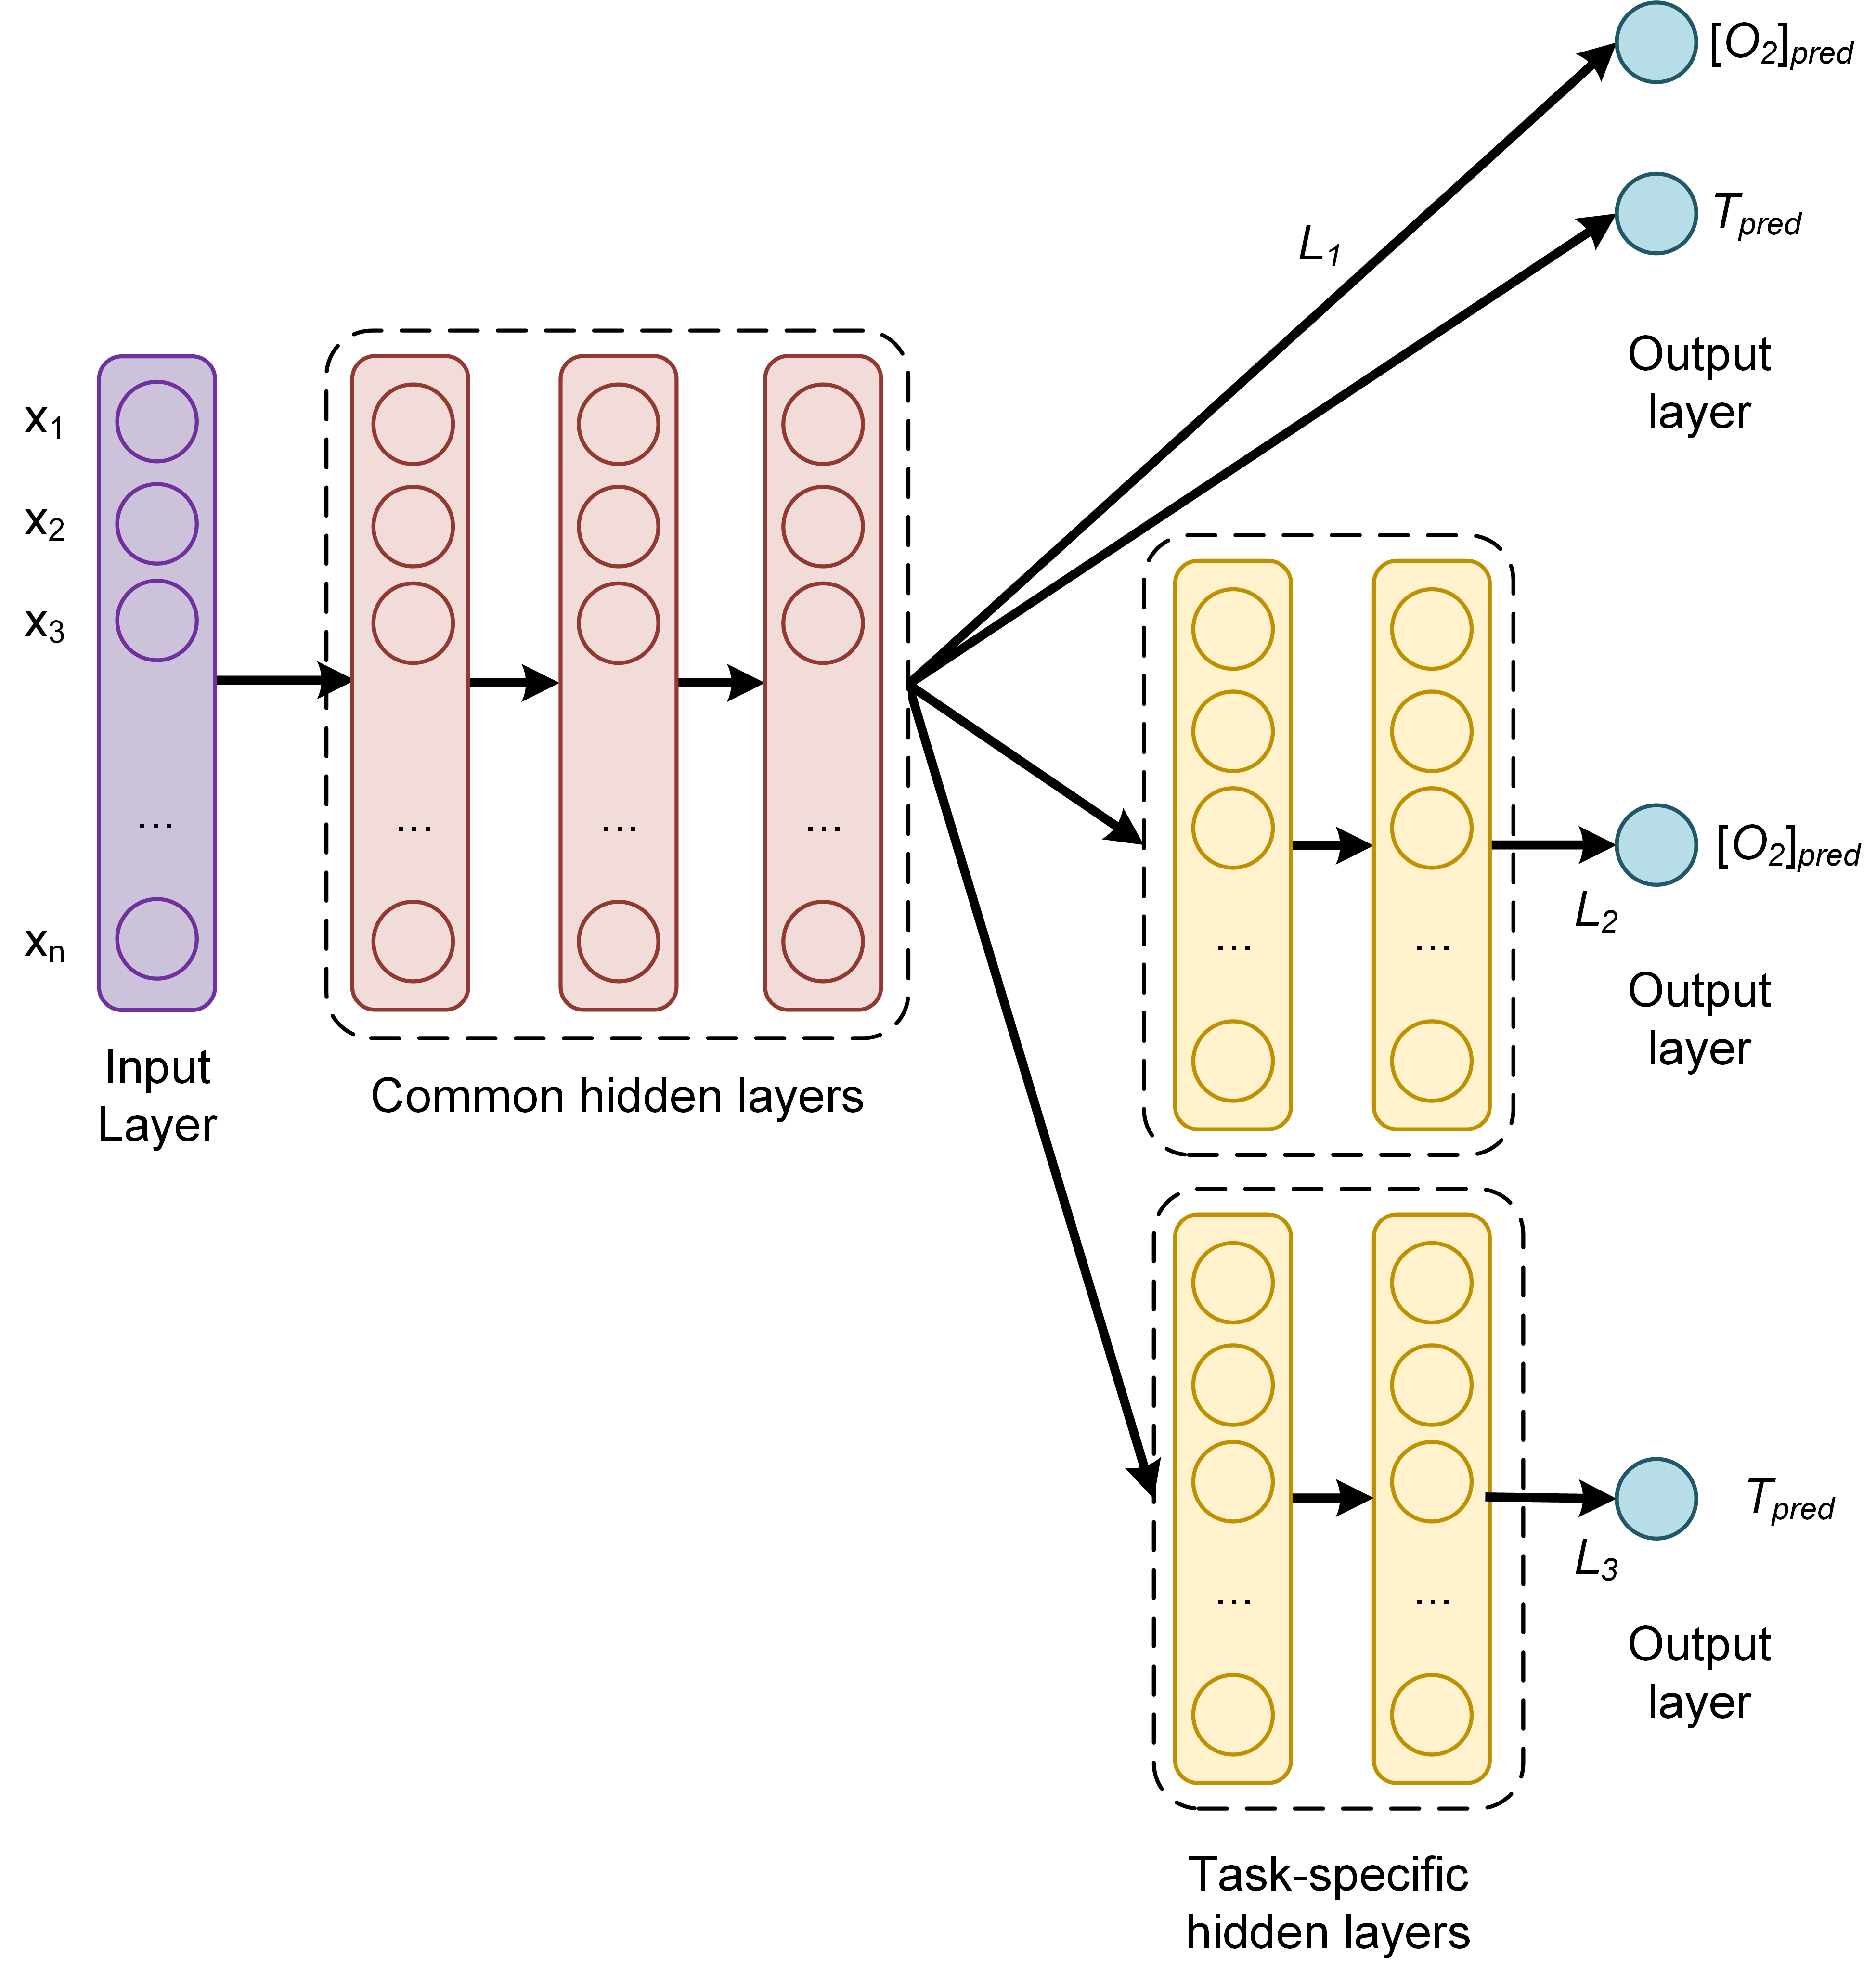
\includegraphics[width=8.7 cm]{NN_MTL_O2_T.png}
\caption{Architecture of the multi-task learning architecture.}
\label{fig:NN_MTL_O2_T}
\end{figure}


\subsubsection{Optimiser Algorithm}

To minimize the cost function, the optimizer Adaptive Moment Estimation (Adam) \cite{Kingma2014, Michelucci2017} was used. The training was performed with a starting learning rate of $10^{-3}$ as mentioned earlier. The neural network has been trained with two methods. 

{\bf No-batch training}:
with this method all the training data to evaluate the cost function is used to perform an update of the weights. The loss function used is the one in Equation (\ref{MSE}) with $n$ is the total number of observations available.

{\bf Mini-batch training}:
with this method a weight update is performed after the network has seen 32 observations. In this case the loss function is the one in Equation (\ref{MSE}) with $n=32$. For each weight update, 32 random observations are chosen from the training dataset without repetitions until all the training dataset has been fed to the network.  

No-batch training has the advantage of stabilty and speed, since it perform one weight update using the entire training dataset \cite{Michelucci2017}. Mini-batch training is normally much more effective, reachine lower values of the loss function in less epochs, but normally takes much more time. In our experimentes No-batch training takes, for $10^3$ epochs roughly 5 minutes on a modern macbook pro, while mini-batch training with $b=32$ takes, for the same amount of epochs, roughly 1 hour, so it is ca. 12 times slower, but is, as it will be shown later, much more effective. 
The implementation was performed using the TensorFlow$\texttrademark$ library. 

\subsubsection{Metrics}

The metric used to compare results from different network models is the absolute error ($AE$) defined as the absolute value of the difference between the predicted and the expected value for a given observation. For the oxygen concentration of the 
$j^{th}$ observation $[O_2]^{[j]}$  the $AE$ is 
\begin{equation}
\label{AE}
AE^{[j]}_{[O_2]} = |[O_2]^{[j]}_{pred}-[O_2]^{[j]}_{meas}|.
\end{equation}

The further quantity used to analyze the performance of the network is the mean absolute error ($MAE$), defined as the average of the absolute value of the difference between the predicted and the expected oxygen concentration or temperature. For example, for the oxygen prediction using the training dataset $S_{train}$, $MAE_{[O_2]}$ is defined as 
\begin{equation}
\label{MAE}
MAE_{[O_2]}(S_{train}) = \frac{1}{|S_{train}|} \sum_{j \in S_{train}}|[O_2]_{pred}^{[j]}-[O_2]_{real}^{[j]}|
\end{equation}
where $|S_{train}|$ is the size (or cardinality) of the training dataset. For example, in this work $|S_{train}|$=20000.
The $AE_{T}$ and $MAE_T$ are similarly defined.

\subsubsection{Error Limited Accuracy}

\section{Results and Discussion}
\label{Results}

\subsection{Luminescence Experimental Results}

As described in Section \ref{Theory}, the phase-shift depends not only on the oxygen concentration, but also on the temperature and on the modulation frequency of the excitation light. This can be seen in the Figs. \ref{fig:expdata1} to \ref{fig:expdata3}.
Fig. \ref{fig:expdata1} shows the measured phase shifts as a function of the oxygen concentration at a constant modulation frequency for increasing temperatures. For clarity, only selected temperatures are shown. The decrease in the phase shift with increasing concentration is the quenching of the luminescence described in Eq. \ref{theta_full}. The effect of the temperature is to further decrease the phase shift but the effect depends on the concentration, being stronger at higher oxygen concentration. This temperature quenching is understandable since higher temperature.... 

\begin{figure}[htbp]
\centering

\includegraphics[width=8 cm]{phase_O2_T.eps}
\caption{Measured phase-shift as a function of the oxygen concentration, for selected temperatures at a fixed modulation frequency of 6 kHz. The arrow marks increasing temperatures.}
\label{fig:expdata1}
\end{figure}

For a given oxygen concentration the phase shift is strongly dependent from the modulation frequency, as it can be seen in Fig. \ref{fig:expdata2}. Again, the temperature quenching is visible and affects the phase shift differently depending on the modulation frequency.

\begin{figure}[htbp]
\centering

\includegraphics[width=8 cm]{phase_f_T.eps}
\caption{Measured phase-shift for selected oxygen concentrations as a function of the modulation frequency at a fixed oxygen concentration $[O_2]=20 \%$ at selected temperatures.}
\label{fig:expdata2}
\end{figure}

The complementary to Fig. Fig. \ref{fig:expdata2} is shown in Fig. \ref{fig:expdata3}, where the phase shift is shown a function of the modulation frequency for selected oxygen concentrations at a fixed temperature.

\begin{figure}[htbp]
\centering

\includegraphics[width=8 cm]{phase_f_O2.eps}
\caption{Measured phase-shift for selected oxygen concentrations as a function of the modulation frequency at a fixed temperature $T=25 ^{\circ}$ .}
\label{fig:expdata3}
\end{figure}

Comparing the curves shown above it is clear that, when measuring one single phase-shift or even a the phase-shift as a function of the modulation frequency is not possible to simultaneously determine both the oxygen concentration and the temperature from this set of data. To determine the oxygen concentration is mandatory to know the temperature. This is no longer the case with the artificial intelligence approach, as it will be shown in the next section. 

\subsection{Sensor performance analysis}

\subsubsection{Kernel Density Estimation}

To analyze the performance of the network, a fundamental quantity is the prediction probability density?? distribution of the $AE$s since it carries information on the probability of the network to predict the expected value.  for each parameter. For this reason the   kernel density estimate (KDE) of the distributions of the $AE$s for both the oxygen concentration and the temperature was calculated. KDE is a non-parametric algorithm to estimate the probability density function of a random variable by inferring the population distribution based on a finite data sample \cite{Hastie2009}. ATTENZIONE COPIATO DA WIKIPEDIA
In this work a Gaussian Kernel and a Scott bandwidth adaptive estimation \cite{Sain1996} using the seaborn Python package \cite{Waskom2020} were used.

\subsubsection{Error Limited Accuracy $\eta$}

To better characterise the sensor performance we need to define a new metric, that we have called Error Limited Accuracy (ELA), and that we indicate with $\eta$. 

\begin{definition}
In a regression problem, given a metric $m$, and a certain value of it $\hat m$, the ELA for this metric $\eta$ is defined as the number of predictions $\hat y$ of the NNM that lie in the range $[y-\hat m, y+\hat m]$. Or in more mathematical terms once we define the set
\begin{equation}
S(\hat m) = \{ \hat y^{[i]} \ {\text with } \ i = 1,..., n\ | |m(\hat y^{[i]})-m(y^{[i]})|\leq \hat m \} 
\end{equation}
$\eta$ can be simply defined as
\begin{equation}
\eta = \frac{|S(\hat m)|}{n}
\end{equation}
where $|S(\hat m)|$ is the cardinality of the set $S(\hat m)$ or in other words, the number of its elements.
\end{definition}


\subsection{Sensor performance}


The results for $AE_{[O_2]}$ and $AE_T$ for are shown in Figure \ref{fig:prediction_distribution_batch_90}.

\begin{figure*}[htbp]
\centering
\includegraphics[width=17 cm]{prediction_distribution_batch.eps}
\caption{Performance of the neural network for the oxygen (left plot) and for the temperature (right plot) predictions: Normalized prediction distribution histogram (columns) and kernel density estimate (KDE) of the distribution of the $AE$s (solid line) using plain gradient descent (GD) and using mini-batches (MB) with a batch size of 32. The corresponding $MAE$ is also shown as a dashed line in each diagram.}
\label{fig:prediction_distribution_batch_90}
\end{figure*}

\begin{figure*}[htbp]
\centering
\includegraphics[width=17 cm]{prediction_distribution_epochs.eps}
\caption{Performance of the neural network for the oxygen (left plot) and for the temperature (right plot) predictions: Normalized prediction distribution histogram (columns) and kernel density estimate (KDE) of the distribution of the $AE$s (solid line) using plain gradient descent (GD) and using mini-batches (MB) with a batch size of 32. The corresponding $MAE$ is also shown as a dashed line in each diagram.}
\label{fig:prediction_distribution_epochs_90}
\end{figure*}

\begin{figure*}[htbp]
\centering
\includegraphics[width=17 cm]{prediction_distribution_theta0.eps}
\caption{Performance of the neural network for the oxygen (left plot) and for the temperature (right plot) predictions: Normalized prediction distribution histogram (columns) and kernel density estimate (KDE) of the distribution of the $AE$s (solid line) using plain gradient descent (GD) and using mini-batches (MB) with a batch size of 32. The corresponding $MAE$ is also shown as a dashed line in each diagram.}
\label{fig:prediction_distribution_theta0}
\end{figure*}

\begin{figure}[htbp]
\centering

\includegraphics[width=7 cm]{ELA_1.eps}
\caption{Phase-shift at a fixed temperature $T=25 ^{\circ}$ for selected oxygen concentrations as a function of the modulation frequency of the excitation light.}
\label{fig:result_theta0}
\end{figure}




Finally, the performance of the different neural networks is summarized in Table \ref{TableMAE_summary}. Here the $MAE$ as defined in Equation \ref{MAE} for the oxygen concentration and the temperature prediction are listed.

\begin{table}[hbt]
\centering
\caption {\bf Summary of the performance for the three types of neural networks}

\begin{tabular}{ rccc}
\smallskip 
 Input & Epochs / Batch size & $MAE_{[O_2]}$ & $MAE_{[T]}$  \\ 
 \hline
$\theta / 90^\circ$ & 20'000 / 4000 & xx \% air & xx $^\circ C$\\ 
$\theta / 90^\circ$ & 20'000 / 32 & xx\% air & xx $^\circ C$\\ 
$\theta / 90^\circ$& 100'000 / 32 & xx \% air & xx $^\circ C$\\ 
$\theta /\theta_0$ & 20'000 / 32 & xx \% air & xx $^\circ C$\\ 

\end{tabular}
\label{TableMAE_summary}
\end{table}



plot theta/theta0 vs frequency for different T (O2 fix) and for different O2 (T fix)
plot distribution of total AE

temperature can be presicted less well because phase shift depends less from T than from O2

Stability results

temperature cannot be predicted well without dividing for theta 0




\section{Conclusions}



%\section*{Funding Information}
%National Science Foundation (NSF) (1263236, 0968895, 1102301); The 863 Program (2013AA014402).

%\section*{Acknowledgments}


\section*{Disclosures}

\medskip

\noindent\textbf{Disclosures.} The authors declare no conflicts of interest.


% Bibliography
\bibliography{bibliography}

% Full bibliography will be added automatically on a new page for Optics Letters submissions. This command is ignored for journal article submissions.
% Note that this extra page will not count against page length.
\bibliographyfullrefs{bibliography}

%\printbibliography

%Manual citation list
%\begin{thebibliography}{1}
%\bibitem{Michelucci2017}
%Michelucci, U.
%{\sl Applied Deep Learning - A Case-Based Approach to Understanding Deep Neural Networks}; Apress Media, LLC: New York, NY, USA, 2018; pp. 374--375.

%\bibitem{Kingma2014}
%Kingma, D.P.; Ba, J.
%Adam: A method for stochastic optimization. In Proceedings of 3rd International Conference on Learning Representations, ICLR 2015, San Diego, CA, USA, May 7-9, 2015, pp. 1--15.

%\bibitem{Michelucci2019}
%Michelucci, U.; Baumgartner, M.; Venturini, F.
%Optical oxygen sensing with artificial intelligence.
%{\sl Sensors} {\bf 2019}, {\sl 19}, 777.

˜
%\bibitem{Zhang:14}
%Y.~Zhang, S.~Qiao, L.~Sun, Q.~W. Shi, W.~Huang, %L.~Li, and Z.~Yang,
 % \enquote{Photoinduced active terahertz metamaterials with nanostructured
  %vanadium dioxide film deposited by sol-gel method,} Opt. Express \textbf{22},
  %11070--11078 (2014).
%\end{thebibliography}

\end{document} 